\begin{knitrout}
\definecolor{shadecolor}{rgb}{0.969, 0.969, 0.969}\color{fgcolor}\begin{kframe}
\begin{alltt}
\hlkwd{set.seed}\hlstd{(}\hlnum{2021}\hlstd{)}
\hlstd{g} \hlkwb{<-} \hlnum{4} \hlcom{# number of groups}
\hlstd{n} \hlkwb{<-} \hlnum{40} \hlcom{# number of instances in each group}
\hlstd{z} \hlkwb{<-} \hlkwd{rep}\hlstd{(}\hlnum{1}\hlopt{:}\hlnum{4}\hlstd{,} \hlkwc{each}\hlstd{=n)} \hlcom{# grouping variable}
\hlstd{x} \hlkwb{<-} \hlkwd{runif}\hlstd{(n}\hlopt{*}\hlstd{g,} \hlnum{0}\hlstd{,} \hlnum{2}\hlstd{)} \hlopt{+} \hlstd{z} \hlcom{# x variable that depends on z}
\hlstd{y} \hlkwb{<-} \hlnum{2} \hlopt{*} \hlstd{z} \hlopt{-} \hlstd{x} \hlopt{+} \hlkwd{rnorm}\hlstd{(n}\hlopt{*}\hlstd{g)} \hlcom{# y variable that depends on x and z}
\hlkwd{plot}\hlstd{(x, y)} \hlcom{# plot the whole data}
\end{alltt}
\end{kframe}\begin{figure}

{\centering 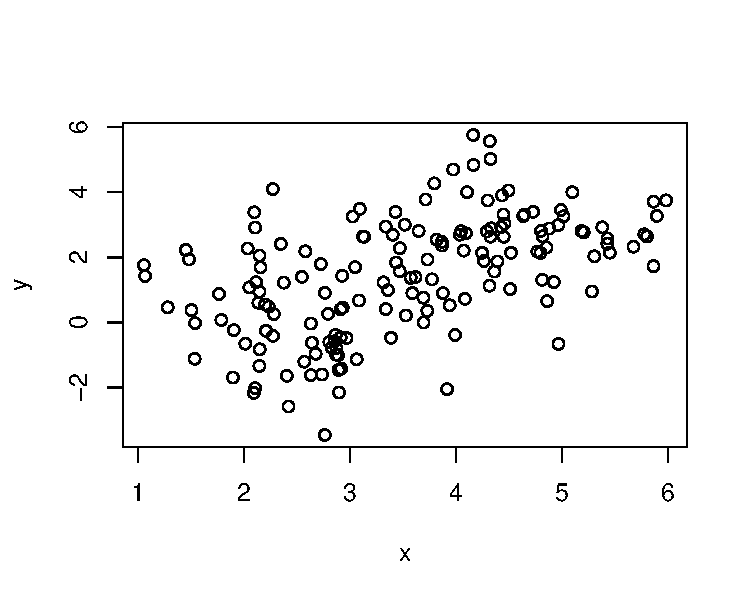
\includegraphics[width=\maxwidth]{figure/probability-Simpson-1} 

}

\caption[Scatter plot for the whole data]{Scatter plot for the whole data}\label{fig:probability-Simpson}
\end{figure}

\end{knitrout}

\begin{knitrout}
\definecolor{shadecolor}{rgb}{0.969, 0.969, 0.969}\color{fgcolor}\begin{kframe}
\begin{alltt}
\hlkwd{plot}\hlstd{(x, y,} \hlkwc{pch}\hlstd{=}\hlkwd{rep}\hlstd{(}\hlnum{1}\hlopt{:}\hlstd{g,} \hlkwc{each}\hlstd{=n),} \hlkwc{col}\hlstd{=}\hlkwd{rep}\hlstd{(}\hlnum{1}\hlopt{:}\hlstd{g,} \hlkwc{each}\hlstd{=n))}
\end{alltt}
\end{kframe}\begin{figure}

{\centering 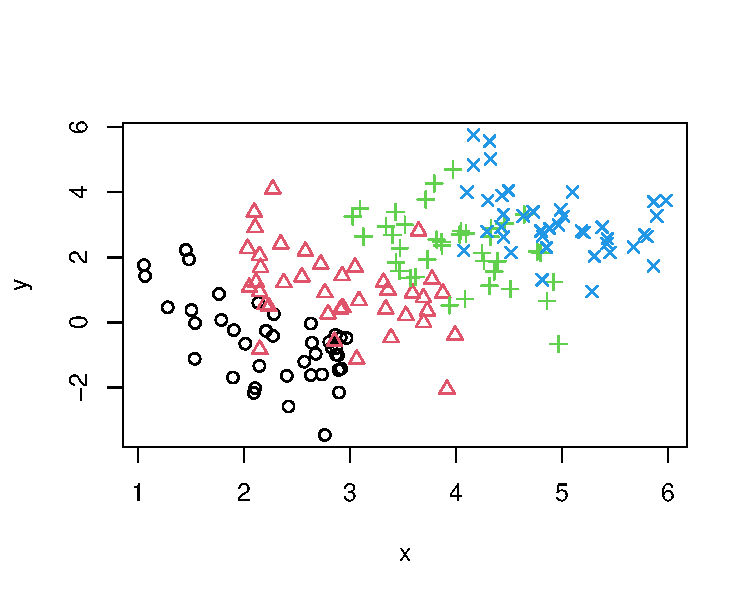
\includegraphics[width=\maxwidth]{figure/probability-Simpson2-1} 

}

\caption[Scatter plot with different groups labeled]{Scatter plot with different groups labeled}\label{fig:probability-Simpson2}
\end{figure}

\begin{kframe}\begin{alltt}
\hlcom{# label the points for different groups}
\end{alltt}
\end{kframe}
\end{knitrout}
